\documentclass{scrartcl}
\usepackage{amsmath}
\usepackage{graphicx}
\begin{document}

	\title{Compte-rendu de travaux pratiques de physique}
	\subtitle{Spectromètre à fibre optique}
	\author{Benjamin Loison et Sara de Francqueville (MPSI 1)}
	\date{24 décembre 2018}
	\maketitle

  \setcounter{section}{1}
	\section{Acquisition de spectres}

		\subsection{Lampe spectrale}

			Dans chacune des lampes spectrales, nous observons respectivement du cadmium (Cd) et du mercure (Hg). Quant aux néons de la salle, nous remarquons une présence de mercure (Hg).
			
		\subsection{Sources lumineuses rouges}

			Dans le premier cas, la largeur à mi-hauteur est de 20.1 nm, dans le cas du laser, la largeur à mi-hauteur est de 1.1 nm. Le laser est encore plus monochromatique que la LED rouge qui présente seulement une largeur à mi-hauteur de 20.1 nm, ce qui la fait paraître d'un rouge monochromatique.
			
			\subsection{Spectre de corps noir}

				\begin{figure}
					\centering
					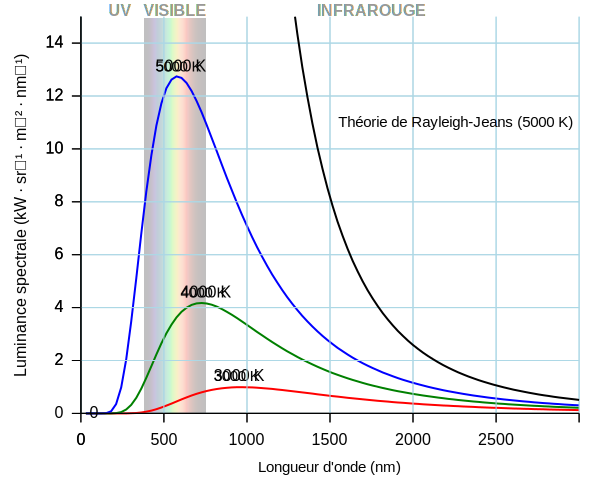
\includegraphics[scale=0.75]{Black_body_fr.png}
					\caption{Corps noir (Wikipedia)}
					\label{fig1}
				\end{figure}
			
			

\end{document}